\chapter{Revisão de literatura e conceituação teórica} \label{cap:conceitos}

Este capítulo tem como objetivo introduzir os conceitos teóricos básicos utilizados no documento e bases para apresentar a método.

\section{Problemas de Decisão} \label{sec:problemaDecisao}

Um problema $\Pi$ é dito um problema de decisão quando seu conjunto solução é composto apenas pelos elementos \textit{Sim} e \textit{Não}, ou seja:
\begin{equation} \label{eq:problemaDecisao}
\begin{split}
\Pi: D \rightarrow Im  \\
Im = \{ Sim, N\widetilde{a}o \}
\end{split}
\end{equation}

São exemplos de problemas de decisão:
\begin{itemize}
    \item{Seja $x \in C$, sendo $x$ um número pertencente ao conjunto $C$, $x$ é o menor número deste conjunto?}
    \item{Seja um grafo $G(V,A)$ denotado pelos arestas $A$ e vértices $V$, existe um caminho do vértice $x$ para o vértice $y$ com custo menor que $c$?}
\end{itemize}

\section{Problemas de Otimização} \label{sec:problemaOtimizacao}

Seja $\Pi$ um problema, S o conjunto de soluções viáveis para o mesmo e $f$ a função objetivo que associa uma solução $s_i$ a um valor numérico então temos:
\begin{equation}  \label{eq:problemaOtimizacao}
\begin{split}
S = \{s_1, s_2, \dots, s_n \} \\
f: S \rightarrow \mathbb{R}
\end{split}
\end{equation}

Um problema de otimização, em geral, pode ser de minimização ou de maximização.
$\Pi$ é um problema de minimização se ele consiste em determinar uma solução $s^*$ tal que:
\begin{equation}  \label{eq:problemaOtimizacaoMinimizar}
s^* \in S \mid f(s^*) \leq f(s), \forall s \in S
\end{equation}

De forma análoga um problema de minimização pode ser dado por:
\begin{equation}  \label{eq:problemaOtimizacaoMaximizar}
s^* \in S \mid f(s^*) \geq f(s), \forall s \in S
\end{equation}

Os problemas de otimização podem ser divididos em dois tipos:

\begin{itemize}
    \item Otimização contínua: nesse tipo de problema pelo menos uma das variáveis $x$ do conjunto de variáveis $X$ pode assumir infinitos valores;
    \item Otimização combinatória: problemas em que toda variável $x$ no conjunto de variáveis $X$ é discreta, podendo assumir apenas um número finito ou infinito porém contável de valores.
\end{itemize}

Desta forma, existe um número finito de soluções viáveis para um problema de otimização combinatória.
Para todo problema de decisão existe um problema de otimização associado, tomemos com exemplo os problemas da seção~\ref{sec:problemaDecisao} e teremos os seguintes problemas de otimização:

\begin{itemize}
    \item Seja um conjunto $C$, encontrar $x \in C \mid x < y, \forall y \in C$.
    \item Seja um grafo $G(V,A)$ denotado pelos arestas $A$ e vértices $V$, encontrar o menor caminho do vértice $x$ para o vértice $y$.
\end{itemize}

\section{Problema da Mínima Latência}\label{sec:mlp}

O Problema da Mínima Latência (PML) é um problema de otimização, sendo uma variante do PCV no qual o objetivo é minimizar o tempo de chegada (ou latência) aos vértices, e não a distância ou tempo da rota como no problema original.
O PML pode ser definido como um grafo direcionado $G=(V,E)$, onde $V=\{0,1,\dots,n\}$ é um conjunto de vértices e $E = \{(i, j) : i, j \in V, i \ne j \}$ um conjunto de arestas que conectam os vértices.
Para cada arco $(i,j)$ existe um tempo de viagem associado igual a $t(i,j)$. O vértice 0 representa o ponto de saída (depósito) e os demais os clientes a serem visitados.
O tempo de chegada (ou latência) a um cliente $i \in V$, é denotado por $l(i)$, o qual é definido pelo tempo de viagem do depósito até o vértice $i$.

\begin{figure}[htpb]
    \centering
    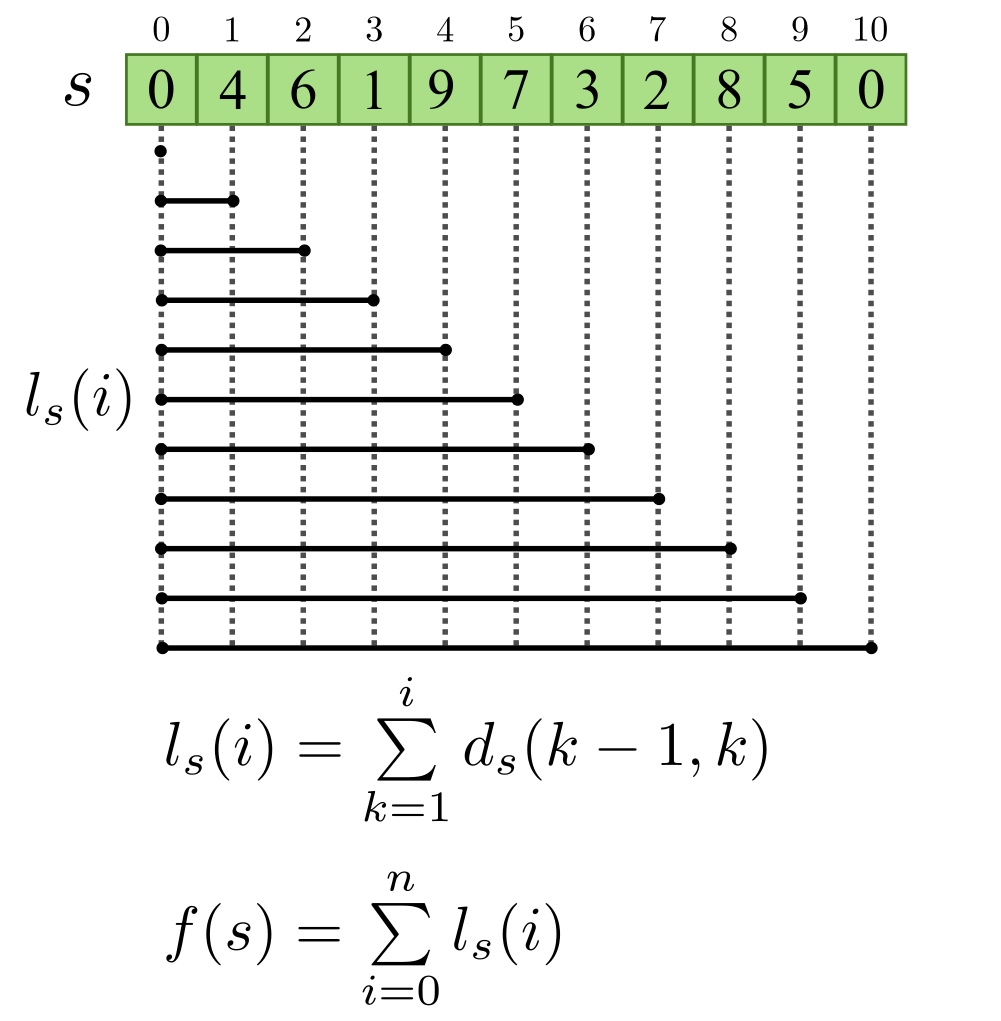
\includegraphics[width=0.6\linewidth]{figuras/pml/mlp}
    \caption{Exemplo de solução com as latências de cada cidade e cálculo da função objetivo}
    \label{fig:pmlDiagramaFormulas}
\end{figure}

O objetivo do PML é, iniciando do depósito, determinar o ciclo Hamiltoniano $s$ que minimize a latência expressa por $L(s)=\sum_{i=0}^{n} l(i)$ como pode ser visto na Figura~\ref{fig:pmlDiagramaFormulas}.
Assim sendo, uma solução viável do PML consiste numa permutação de $n$ clientes determinando a ordem de visita dos mesmos. Tomemos o exemplo a seguir, se $n=9$,  $s=[0,8,3,7,1,4,2,5,6,0]$ é uma solução viável para o PML (de fato, qualquer permutação $1..8$ começando e terminando no vértice zero é uma solução viável).

Apesar da formulação simples e de sua grande aplicação na otimização de latência em redes, o PML é um problema complexo, sendo provado que o PML é NP-Difícil~\cite{silva2012}. A despeito da semelhança na formulação do PML com a do Problema do Caixeiro Viajente (PCV) a sua função objetivo é mais complexa de ser calculada que a do PCV.
No PML, pequenas alterações no vetor solução podem levar a grandes alterações no resultado final da solução e a natureza não local da função objetivo faz com que uma simples inserção afete todas as latências subsequentes.
Na literatura, o PML também é conhecido Problema do Caixeiro Viajante Cumulativo \cite{bianco1993}, Problema do Entregador \cite{mladenovic2013} e Problema do Reparador Viajante. \cite{tsitsiklis1992}.

Em trabalhos recentes, um procedimento de busca local baseado em \emph{Graphics Processing Unit} (\emph{GPU}) e computação \emph{multi-core} foi proposto para o PML~\cite{wamca2016}.
A ideia foi chamada \emph{Distributed Variable Neighborhood Descent} (\emph{DVND}), tentando explorar diferentes estratégias de vizinhança simultaneamente para uma solução de entrada.

Em otimização, uma vizinhança é definida como um conjunto de operações chamados "movimentos", que são capazes de realizar pequenas alterações na solução de entrada.
Estas alterações podem ser, por exemplo, trocar dois elemento na permutação inicial, gerando dessa forma $\mathcal{O}(N^2)$ diferentes soluções (para o caso de uma permutação de tamanho $N$). Existe na literatura muitas dessas vizinhanças (como 2-Opt, OrOpt-1, OrOpt-2, Swap, ..., etc), conquanto por limitações computacionais estes são sempre explorados de forma sequencial, chamados de \emph{Variable Neighborhood Descent} (\emph{VND}).
Com o objetivo de encontrar um ótimo local para o PML, a ideia principal do DVND é usar GPU para obter operações de grão fino (que em geral são rápidas) e explorar toda a vizinhança $\mathcal{O}(N^2)$ mais rápido que em CPU (como explicado em~\cite{wamca2016}) e combinar as respostas das buscas, escolhendo a nova melhor solução.

% \subsection{Exemplo}

% \begin{figure}[htpb]
%     \centering
%     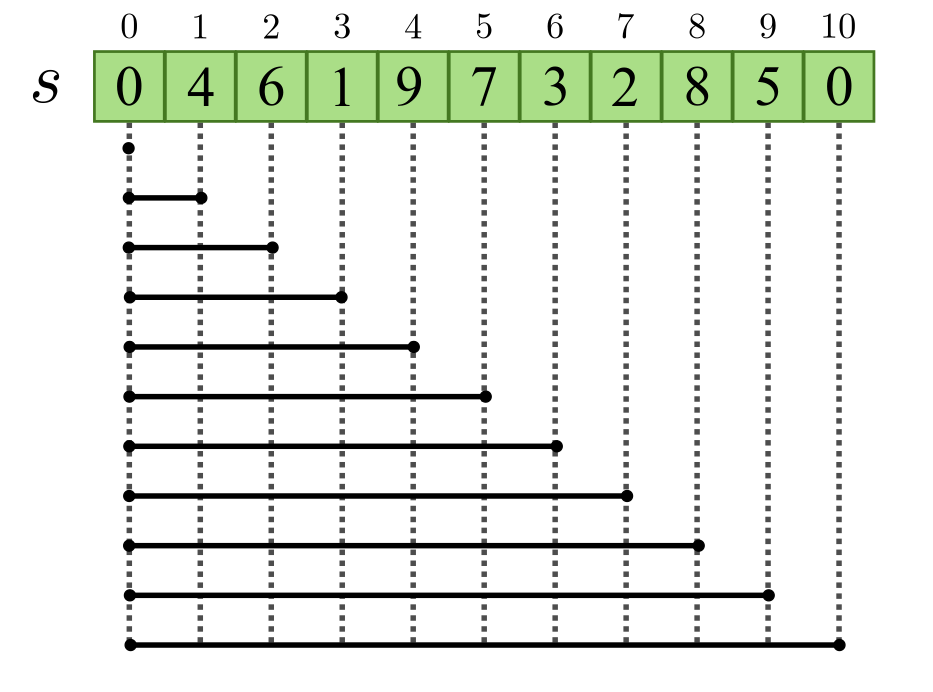
\includegraphics[width=0.6\linewidth]{figuras/pml/mlp-clean}
%     \caption{Exemplo de solução com as latências de cada cidade}
%     \label{fig:pml}
% \end{figure}

Pelo exemplo na Figura~\ref{fig:pmlDiagramaFormulas} podemos ver que o valor da latência $L(s)$ será dado palos somatórios das latências de todas as cidades, sendo $d_s^{i, j}$ a distância da cidade $i$ para a cidade $j$ na solução $s$, então temos:
$$ L(s) = \sum_{i=0}^n{l_s(i)} $$
$$ L(s) = l_s(0) + l_s(1) + l_s(2) + l_s(3) + l_s(4) + l_s(5) + l_s(6) + l_s(7) + l_s(8) + l_s(9) $$
$$ L(s) = 10d_s^{0, 4} + 9d_s^{4, 6} + 8d_s^{6, 1} + 7d_s^{1, 9} + 6d_s^{9, 7} + 5d_s^{7, 3} + 4d_s^{3, 2} + 3d_s^{2, 8} + 2d_s^{8, 5} + d_s^{5, 0}$$

\section{Busca local} \label{sec:buscaLocal}

Um algoritmo de busca local percorre iterativamente o espaço de soluções de um determinado problema melhorando a solução atual.
Para tanto procura na vizinhança (definida na Seção~\ref{subsec:vizinhanca}) atual por uma solução melhor que a atual e repete o processo até não ser encontrada uma melhora.

\subsection{Vizinhança} \label{subsec:vizinhanca}

Seja $S$ o espaço de soluções de um problema de otimização $\Pi$, e $s \in S$ uma solução qualquer, considere a função objetivo $f: S \rightarrow \mathbb{R}$ que atribui um valor para cada solução.
Denotamos então por $N^x(s)$ o conjunto de soluções vizinhas de $s$ para a vizinhança $x$ com $N^x(s) \subseteq S$, em que as soluções dessa vizinhança podem ser obtidas de $s$ a partir da aplicação de determinadas operações.
Uma solução $s'$ é vizinha de $s$ (isto é $s' \in N^x(s)$) segundo uma vizinhança $s$ se $s'$ é alcançável a partir de $s$ fazendo uso de uma pequena perturbação nesta última.

\subsection{Movimento} \label{subsec:movimento}

% Seja $S$ o espaço de soluções de um problema de otimização $\Pi$, e $s \in S$ uma solução qualquer, considere a função objetivo $f: S \rightarrow \mathbb{R}$ que atribui um valor para cada solução.
Considere $m^k: S \rightarrow S$ a função que representa um movimento que leva uma solução $s$ a uma solução $s'$ ou de forma equivalente $s' = m^k \circ s$.
Designamos então o movimento $m^k \in M^k$ no conjunto de movimentos da vizinhança $k$.

Adicionalmente podemo definir o custo do movimento $m^k(s)$ em relação a solução $s$ como sendo a diferença entre o valor da solução $s'$ gerada ao aplicar este movimento à solução $s$ e o valor da solução $s$, conforme pode ser visto na Equação~\ref{eq:movimentoCusto}, iremos omitir a função $f$ e a vizinhança $k$ quando estiverem claros no contexto, desta forma a podemmos simplificar a notação conforme a Equação~\ref{eq:movimentoCustoSimplificada}.
Formalmente, a notação circunflexo representa a função $\widehat{m}: S \rightarrow \mathbb{R}$.
\begin{equation} \label{eq:movimentoCusto}
\widehat{m^k_f}(s) = f(s') - f(s)
\end{equation}

\begin{equation} \label{eq:movimentoCustoSimplificada}
\widehat{m^k_f}(s) = \widehat{m}(s) = f(s') - f(s)
\end{equation}

Para exemplificar as definições que se seguem tomemos a Tabela~\ref{tab:coordenadasComMatrizDistancias}, consideremos um conjunto de cidades com suas localizações conforme a Tabela~\ref{tab:coordenadasCidades}.
Para facilitar o acompanhamento considere a matriz de distâncias expressa na Tabela~\ref{tab:distanceMatrix}.

\begin{table}[ht]
    \centering
    \begin{subtable}{.3\textwidth}
    \centering
    \begin{tabular}{c|cc}
    	\hline
    	Cidade & $x$ & $y$ \\
    	\hline
    	A &	200 &	200 \\
    	B &	100 &	400 \\
    	C &	200 &	800 \\
    	D &	400 &	900 \\
    	E &	600 &	700 \\
    	F &	900 &	600 \\
    	G &	1000 &	400 \\
    	H &	700 &	100 \\
    	I &	500 &	200 \\
    	\hline
    \end{tabular}
    \caption{Coordenadas das cidades.}
    \label{tab:coordenadasCidades}
    \end{subtable}% <---- don't forget this %
    \begin{subtable}{.675\textwidth}
    \centering
    \begin{tabular}{c|ccccccccc}
    	\hline
    	   &   A&   B&   C&   D&   E&   F&   G&   H&   I\\
    	\hline
    	 A &    & 224& 600& 728& 640& 806& 825& 510& 300\\
    	 B & 224&    & 412& 583& 583& 825& 900& 671& 447\\
    	 C & 600& 412&    & 224& 412& 728& 894& 860& 671\\
    	 D & 728& 583& 224&    & 283& 583& 781& 854& 707\\
    	 E & 640& 583& 412& 283&    & 316& 500& 608& 510\\
    	 F & 806& 825& 728& 583& 316&    & 224& 539& 566\\
    	 G & 825& 900& 894& 781& 500& 224&    & 424& 539\\
    	 H & 510& 671& 860& 854& 608& 539& 424&    & 224\\
    	 I & 300& 447& 671& 707& 510& 566& 539& 224& \\
    	 \hline
    \end{tabular}
    \caption{Matriz de distâncias euclidianas com valores inteiros arredondados.}
	\label{tab:distanceMatrix}
    \end{subtable}
\caption{Informações de distâncias e localização das cidades para os exemplos apresentados.}
\label{tab:coordenadasComMatrizDistancias}
\end{table}

Tomemos como exemplo a solução $s_1$ expressa na Figura~\ref{fig:figuraExemplo_s1}, este apresenta uma solução para o problema apresentado na Tabela~\ref{tab:coordenadasComMatrizDistancias} com valor de função objetivo 2631 para o PCV e 13074 para o PML.

\begin{figure}[ht]
    \begin{minipage}{.475\textwidth}
        \begin{subfigure}[t]{1\textwidth} %
            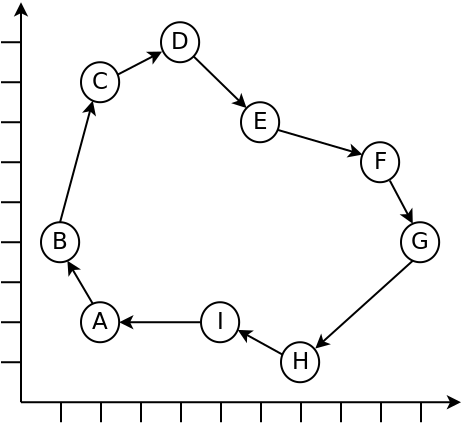
\includegraphics[width=1\linewidth]{figuras/pml/exemplo-rodolfo-opt.png}
        \end{subfigure}
    \end{minipage}
    \begin{minipage}{.475\textwidth}
\begin{Verbatim}[commandchars=\\\{\}]
index:   0  1  2  3  4  5  6  7  8
cidade:  A  B  C  D  E  F  G  H  I
\end{Verbatim}
\begin{gather*}
    f(s_1): 2631/13074 \ (PCV/PML)
\end{gather*}
    \end{minipage}
    \caption{Solução $s_1$.}
    \label{fig:figuraExemplo_s1}
\end{figure}

Ao aplicarmos à solução anterior $s_1$ o movimento $m_1$ 2-opt(1,7), exibido na Figura~\ref{fig:figuraExemplo_m1s1}, este reverte bloco de 1 a 7 (remove implicitamente duas arestas e reconecta a rota), o custo do movimento é $\widehat{m_1}(s_1)$: 509 para o PCV e 3113 para o PML.

\begin{figure}[ht]
    \begin{minipage}{.475\textwidth}
        \begin{subfigure}[t]{1\textwidth} %
            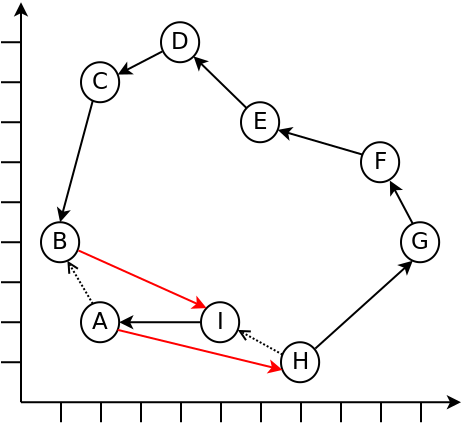
\includegraphics[width=1\linewidth]{figuras/pml/exemplo-rodolfo-2opt-1-7.png}
        \end{subfigure}
    \end{minipage}
    \begin{minipage}{.475\textwidth}
\begin{Verbatim}[commandchars=\\\{\}]
index:  0  1  2  3  4  5  6  7  8
cidade: A  \textcolor{red}{H  G  F  E  D  C  B}  I
\end{Verbatim}
\begin{gather*}
f(m_1 \circ s_1) = 3140/16187 \ (PCV/PML) \\ 
\widehat{m_1}(s_1)+f(s_1) = \\ 
509 + 2631 = 3140 \ (PCV)\\
3113 + 13074 = 16187 \ (PML)
\end{gather*}
    \end{minipage}
    \caption{Solução $m_1 \circ s_1$, com $m_1$ sendo 2-opt(1,7).}
    \label{fig:figuraExemplo_m1s1}
\end{figure}

Outra opção seria escolher o movimento $m_2$ 2-opt(5,6) para ser aplicado à solução, este reverte bloco de 5 a 6 (remove implicitamente duas arestas e reconecta rota), neste caso o custo do movimento é $\widehat{m_2}(s_1)$: 299/1265 para o PCV e PML respectivamente, em detalhes na Figura~\ref{fig:figuraExemplo_m2s1}.

\begin{figure}[ht]
    \begin{minipage}{.475\textwidth}
        \begin{subfigure}[t]{1\textwidth} %
            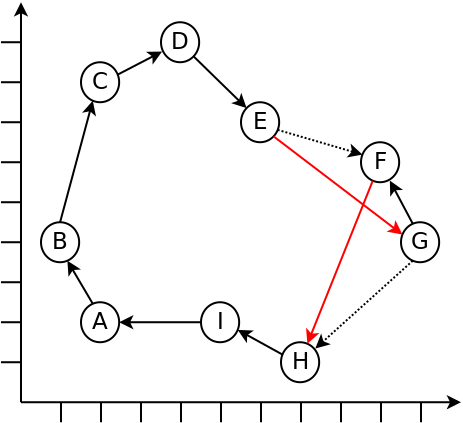
\includegraphics[width=1\linewidth]{figuras/pml/exemplo-rodolfo-2opt-5-6.png}
        \end{subfigure}
    \end{minipage}
    \begin{minipage}{.475\textwidth}
\begin{Verbatim}[commandchars=\\\{\}]
index:   0  1  2  3  4  5  6  7  8
cidade:  A  B  C  D  E  \textcolor{blue}{G  F}  H  I
\end{Verbatim}
\begin{gather*}
f(m_2 \circ s_1): 2930/14339 \ (PCV/PML) \\
\widehat{m_2}(s_1)+f(s_1) = \\
299 + 2631 = 2930 \ (PCV) \\
1265 + 13074 = 14339 \ (PML)
\end{gather*}
    \end{minipage}
    \caption{Solução $m_2 \circ s_1$, com $m_2$ sendo 2-opt(5,6).}
    \label{fig:figuraExemplo_m2s1}
\end{figure}

Adicionalmente se pode ver que a Figura~\ref{fig:figuraExemplo_m3s1} mostra o movimento $m_3$ 2-opt(1,3) sendo aplicado à solução $s_1$, este reverte bloco de 1 a 3 (remove implicitamente duas arestas e reconecta rota) e apresenta um custo de $\widehat{m_3}(s_1)$: 804/6148 para o PCV e PML.

\begin{figure}[ht]
    \begin{minipage}{.475\textwidth}
        \begin{subfigure}[t]{1\textwidth} %
            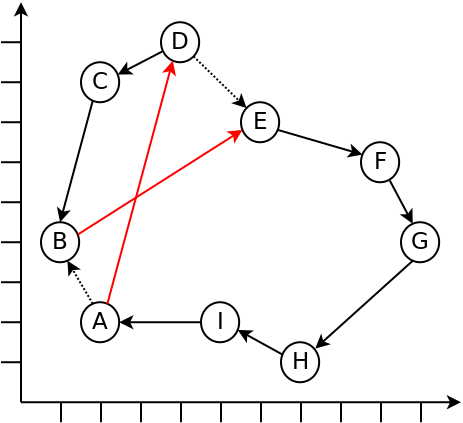
\includegraphics[width=1\linewidth]{figuras/pml/exemplo-rodolfo-2opt-1-3.png}
        \end{subfigure}
    \end{minipage}
    \begin{minipage}{.475\textwidth}
\begin{Verbatim}[commandchars=\\\{\}]
index:   0  1  2  3  4  5  6  7  8
cidade:  A  \textcolor{green}{D  C  B}  E  F  G  H  I
\end{Verbatim}
\begin{gather*}
f(m_3 \circ s_1): 3435/19222 \ (PCV/PML) \\
\widehat{m_3}(s_1)+f(s_1) = \\
804 + 2631 = 3435 \ (PCV)\\
6148 + 13074 = 19222 \ (PML)
\end{gather*}
    \end{minipage}
    \caption{Solução $m_3 \circ s_1$, com $m_3$ sendo 2-opt(1,3).}
    \label{fig:figuraExemplo_m3s1}
\end{figure}

\subsubsection{Movimentos livres de estrutura -- \emph{structure-free moves}} \label{subsubsec:movimentosLivresDeContexto}

Quando a estrutura de armazenamento interna utilizada para representar uma solução permite a aplicação de um movimento para qualquer solução temos um movimento livre de estrutura.
Em outras palavras, um movimento $m$ é livre de estrutura se ele sempre pode ser aplicado a uma solução $s$ sem gerar uma solução inválida.

\begin{equation} \label{eq:movimentoLivreDeContexto}
m \ \textrm{é livre de estrutura} \  \iff m \circ s \in S, \forall s \in S
\end{equation}

Quando uma classe de movimentos é livre de estrutura para um determinado problema então se pode dizer que a função a representar este movimento é fechada para o conjunto de soluções $S$.

A caracterização de um movimento como livre de estrutura depende de suas restrições e da sua representação.
Desta forma, para o Problema do Caixeiro Viajante em que o grafo com as distâncias entre as cidades é completo, o movimento \textit{Swap} será livre de estrutura contudo num grafo incompleto uma aplicação do \textit{Swap} pode gerar uma solução inviável pois pode não existir um determinado percurso após a alteração na solução.

\subsubsection{Movimentos fracamente independentes -- \emph{weakly independent moves}} \label{subsubsec:movimentosParcialmenteIndependentes}

Dois movimentos $\{m_2,m_3\} \subseteq \mathcal{I}$ são fracamente independentes quando a aplicação de um deles não altera o custo do outro movimento para apenas um dos movimentos.
Formalmente temos que dois movimentos $m_1$ e $m_2$ são parcialmente independentes, ou seja $m_1 \parallel_p m_2$, se e somente se:
\begin{equation}
% \begin{align}
m_1 \parallel_p m_2 \iff \widehat{m_1}(s) = \widehat{m_1}(m_2 \circ s)
\label{eq:movimentosParcialmenteIndependentes}
% \end{align}
\end{equation}

\begin{corolario}
Se dois movimentos são parcialmente independentes então o valor da solução resultante será a soma do valor da solução inicial com o custo dos movimentos.

Formalmente temos:
\begin{equation}
m_1 \parallel_p m_2 \implies f(m_1 \circ m_2 \circ s) = \widehat{m_1}(s) + \widehat{m_2}(s) + f(s)
\end{equation}

\begin{proof}
Pela definição de custo do movimento (Equação~\ref{eq:movimentoCusto}) temos:
\begin{align*}
f(m_1 \circ m_2 \circ s) = \widehat{m_1}(m_2 \circ s) + f(m_2 \circ s) & \textrm{ Aplicando Equação~\ref{eq:movimentoCusto}} \\
f(m_1 \circ m_2 \circ s) = \widehat{m_1}(m_2 \circ s) + \widehat{m_2}(s) + f(s) &
\end{align*}

Aplicando-se a definição de movimentos parcialmente independentes temos que:
\begin{align*}
\widehat{m_1}(m_2 \circ s) = \widehat{m_1}(s) & \textrm{ Logo}\\
f(m_1 \circ m_2 \circ s) = \widehat{m_1}(s) + \widehat{m_2}(s) + f(s) + f(s) & \\
\end{align*}
\end{proof}
\end{corolario}

Note que a definição não permite comutatividade, logo nada pode ser afirmado para o caso da solução $m_2 \circ m_1 \circ s$.

Acompanhando o exemplo, se movimentos $m_1$ e $m_2$ forem parcialmente independentes temos:
\begin{gather*}
(m_1 \circ m_2 \circ s_1) = 3439/17452 \\
(m_1 \circ m_2 \circ s_1)= \widehat{m_1}(s_1) + \widehat{m_2}(s_1) + f(s_1) = \\ \\
(m_1 \circ m_2 \circ s_1) = \\
509 + 299 + 2631 = 3439 \ (PCV)\\
3113+1265+13074 = 17452 \ (PML)
\end{gather*}

\begin{figure}[ht]
    \begin{minipage}{.475\textwidth}
        \begin{subfigure}[t]{1\textwidth} %
            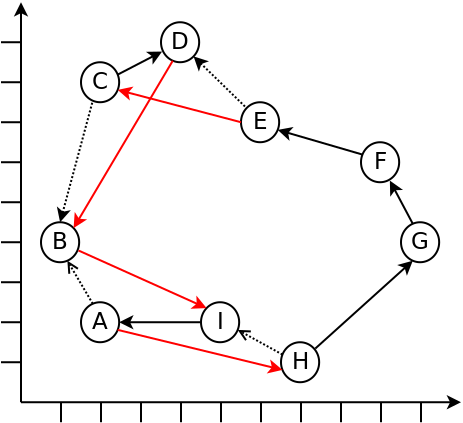
\includegraphics[width=1\linewidth]{figuras/pml/exemplo-rodolfo-2opt-1-7-5-6.png}
        \end{subfigure}
    \end{minipage}
    \begin{minipage}{.475\textwidth}
\begin{Verbatim}[commandchars=\\\{\}]
index:   0  1  2  3  4  5  6  7  8
cidade:  A  \textcolor{red}{H  \textcolor{blue}{F  G}  E  D  C  B}  I
\end{Verbatim}
\begin{gather*}
f(m_1 \circ m_2 \circ s_1)= 3439/18211 \ (PCV/PML) \\
f(m_1 \circ m_2 \circ s_1) = \\
\widehat{m_1}(m_2 \circ s_1) + \widehat{m_2}(s_1) + f(s_1) = \\
509 + 299 + 2631 = 3439 \ (PCV) \\
3872 + 1265 + 13074 = 18211 \ (PML)
\end{gather*}
    \end{minipage}
    \caption{Solução $m_1 \circ m_2 \circ s_1$, com $m_1$ sendo 2-opt(1,7) e $m_2$ sendo 2-opt(5,6).}
    \label{fig:figuraExemplo_m1m2s1}
\end{figure}

Conforme supracitado e ilustrado nas Figuras~\ref{fig:figuraExemplo_m1m2s1} e~\ref{fig:figuraExemplo_m2m1s1} podemos ver que a solução $m_2 \circ m_1 \circ s_1$ não verifica as mesmas propriedades pois apenas $m_1$ não é alterado por $m_2$, desta forma estes movimentos são parcialmente independentes.

\begin{figure}[ht]
    \begin{minipage}{.475\textwidth}
        \begin{subfigure}[t]{1\textwidth} %
            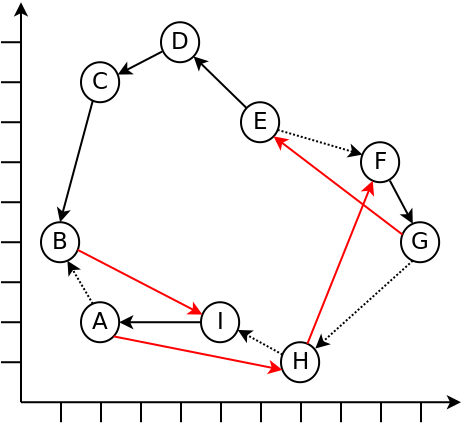
\includegraphics[width=1\linewidth]{figuras/pml/exemplo-rodolfo-2opt-5-6-1-7.png}
        \end{subfigure}
    \end{minipage}
    \begin{minipage}{.475\textwidth}
\begin{Verbatim}[commandchars=\\\{\}]
index:   0  1  2  3  4  5  6  7  8
cidade:  A  \textcolor{red}{H  G  F  E  \textcolor{blue}{C  D}  B}  I
\end{Verbatim}
\begin{gather*}
f(m_2 \circ m_1 \circ s_1) = 3440/17345 \ (PCV/PML) \\
f(m_2 \circ m_1 \circ s_1) = \\
\widehat{m_2}(m_1 \circ s_1) + \widehat{m_1}(s_1) + f(s_1) = \\
300 + 509 + 2631= 3440 \ (PCV) \\
1158 + 3113 + 13074 = 17345) \ (PML)
\end{gather*}
    \end{minipage}
    \caption{Solução $m_2 \circ m_1 \circ s_1$, com $m_2$ sendo 2-opt(5,6) e $m_1$ sendo 2-opt(1,7).}
    \label{fig:figuraExemplo_m2m1s1}
\end{figure}

De fato podemos verificar pela Figura~\ref{fig:figuraExemplo_m2m1s1} que $\widehat{m_2}(s_1)$ = 299/1265 é diferente de $\widehat{m_2}(m_1 \circ s_1)$ = 300/1158.

\subsubsection{Movimentos independentes} \label{subsubsec:movimentosIndependentes}

Movimentos independentes são aqueles que a aplicação de um não altera o valor do outro, o valor do movimento $m_2$ aplicado à solução $m_1 \circ s$ é igual ao valor deste aplicado à solução $s$, a independência de movimentos pode ser definida para movimentos de vizinhanças diferentes.
Em outras palavras movimentos independentes são parcialmente independentes para ambos os lados.
Formalmente temos que dois movimentos $m_1$ e $m_2$ são independentes $m_1 \parallel m_2$ se e somente se:
\begin{equation}
% \begin{align}
m_1 \parallel m_2 \iff \widehat{m_1}(m_2 \circ s) = \widehat{m_1}(s) \;\;\; \land \;\;\; \widehat{m_2}(m_1 \circ s) = \widehat{m_2}(s)
% \end{align}
\end{equation}

\begin{theorem}%[Teorema da independência de movimentos]\label{teo:independenciaMovimentos}
Dois movimentos $m_1$ e $m_s$ são independentes então o valor da solução final não se altera ao alternar a ordem de aplicação dos movimentos, ou seja:
\begin{equation}
m_1 \parallel m_2 \implies f(m_1 \circ m_2 \circ s) = f(m_2 \circ m_1 \circ s)
\end{equation}

\begin{proof}
    Suponhamos que $m_1$ e $m_2$ sejam independentes $\widehat{m_1}(m_2 \circ s) = \widehat{m_2}(s) \land \widehat{m_2}(m_1 \circ s) = \widehat{m_1}(s)$ mas $f(m_1 \circ m_2 \circ s) \neq f(m_1 \circ m_1 \circ s)$.
    \begin{align*}
        f(m_1 \circ m_2 \circ s) \neq & f(m_2 \circ m_1 \circ s) & \textrm{ De }(\ref{eq:movimentoCusto}) \\
        \widehat{m_1}(m_2 \circ s) + f(m_2 \circ s) \neq & \widehat{m_2}(m_1 \circ s) + f(m_1 \circ s) & \textrm{ De }\ (\ref{eq:movimentoCusto}) \\
        \widehat{m_1}(m_2 \circ s) + \widehat{m_2} + f(s) \neq & \widehat{m_2}(m_1 \circ s) + \widehat{m_1} + f(s) & \textrm{ Como } m_1 \parallel m_2 \\
        \widehat{m_1}(s) + \widehat{m_2} + f(s) \neq & \widehat{m_2}(s) + \widehat{m_1} + f(s) & \textrm{ Logo uma contradição } \bot
    \end{align*}
    
    Assim, por \textit{reductio ad absurdum}, temos que se $m_1$ e $m_2$ são independentes então $f(m_1 \circ m_2 \circ s) = f(m_2 \circ m_1 \circ s)$.
\end{proof}
\end{theorem}

Outra propriedade interessante pode ser vista no teorema apresentado a seguir:
\begin{theorem}[Teorema da independência dos movimentos dois a dois]\label{teo:independenciaMovimentos2a2}
Se $m_1 \parallel m_2$ então o valor da solução gerada pela aplicação destes movimentos será igual ao valor anterior da solução somado ao valor dos movimentos.
\begin{equation}
\label{eq:movimentoCustoSomaDois}
m_1 \parallel m_2 \implies f(m_1 \circ m_2 \circ s) = \widehat{m_1}(s) + \widehat{m_2}(s) + f(s)
\end{equation}
\begin{proof}
    Suponhamos que $m_1$ e $m_2$ sejam independentes mas $f(m_1 \circ m_2 \circ s) \neq \widehat{m_1}(s) + \widehat{m_2}(s) + f(s)$.
    \begin{align*}
        f(m_1 \circ m_2 \circ s) \neq & \widehat{m_1}(s) + \widehat{m_2}(s) + f(s) & \textrm{ De } (\ref{eq:movimentoCusto}) \\
        \widehat{m_1}(m_2 \circ s) + f(m_2 \circ s) \neq & \widehat{m_1}(s) + \widehat{m_2}(s) + f(s) & \textrm{ De } (\ref{eq:movimentoCusto}) \\
        \widehat{m_1}(m_2 \circ s) + \widehat{m_2}(s) + f(s) \neq & \widehat{m_1}(s) + \widehat{m_2}(s) + f(s) & \textrm{ Como } m_1 \parallel m_2 \\
        \widehat{m_1}(s) + \widehat{m_2}(s) + f(s) \neq & \widehat{m_1}(s) + \widehat{m_2}(s) + f(s) & \textrm{ Logo uma contradição } \bot
    \end{align*}
    
    Assim, por \textit{reductio ad absurdum}, temos que se $m_1$ e $m_2$ são independentes então $f(m_1 \circ m_2 \circ s) = \widehat{m_1}(s) + \widehat{m_2}(s) + f(s)$.
\end{proof}
\end{theorem}

\subsubsection{Movimentos fortemente independentes -- \emph{strongly independent moves}} \label{subsubsec:movimentosEstritamenteIndependentes}

Dois movimentos $m_1$ e $m_2$ são fortemente independentes quando são independentes e podem ser aplicados simultaneamente a uma solução sem que a alteração feita por um gere conflito na causada pelo outro, a independência de movimentos pode ser definida para movimentos de vizinhanças diferentes.
Formalmente temos que dois movimentos $m_1$ e $m_2$ são fortemente independentes $m_1 \parallel_e m_2$ se e somente se:
\begin{equation}  \label{eq:movimentosIndependentes}
m_1 \parallel_e m_2 \iff m_1(m_2(s)) = m_2(m_1(s)) = m_1 \circ m_2 \circ s = m_2 \circ m_1 \circ s
\end{equation}

% A mesma ideia pode ser aplicada para um conjunto de movimentos $M = \{ m_1, m_2, m_3, ...\}$, são ditos fortemente independentes se para uma solução $s$ qualquer e para todo subconjunto não-vazio $M' = \{ m_1, m_2, m_3, \dots, m_k \} \subseteq M$ temos $m_1 \circ m_2 \circ m_3 \circ ...\circ m_k \circ s = m_2 \circ m_1 \circ m_3 \circ ...\circ m_k \circ s$ para qualquer permutação dos movimentos em $M'$.
% $\widehat{m_1}(s) + \widehat{m_2}(s) + \widehat{m_3}(s) + \dots + \widehat{m_k}(s) = \widehat{m_1}(m_2 \circ m_3 \circ ...\circ m_k \circ s)$. 

Pela Equação~\ref{eq:movimentosIndependentes} pode-se perceber que movimentos fortemente independentes são operações comutativas, pela própria definição.

Assim podemos estender a definição da vizinhança $k$ para:
\begin{equation}  \label{eq:vizinhanca}
N^k(s) = \{ m^k_i \circ s \mid \forall m^k_i \in M^k \}
\end{equation}

Cabe aqui destacar que a independência de movimentos é uma relação dada dois a dois entre os movimentos, logo não existe transitividade na relação de independência destes, ou seja, se temos dois movimentos independentes $m_1 \parallel m_2$ e outro movimento $m_3$ tal que $m_2 \parallel m_3$ então \textbf{não} implica que $m_1 \parallel m_3$.
Pode existir um conflito, logo os movimentos $m_1 \nparallel m_3$ ou seja, seriam conflitantes.
Assim em termos de conflitos entre movimentos podemos escrever:
\begin{equation}
m_1 \parallel m_2 \land m_2 \parallel m_3 \centernot\implies m_1 \parallel m_3
\end{equation}

\begin{proof}
Consideremos o seguinte contraexemplo a seguir para a vizinhança de Swap, sendo os movimentos $Swap(2,3), Swap(3,6), Swap(4,5)$, neste caso podemos ver que $Swap(2,3) \parallel Swap(4,5)$ e que $Swap(4,5) \parallel Swap(3,6)$ contudo $Swap(2,3) \nparallel Swap(3,6)$.
\end{proof}

% Para fins dessa dissertação, por questão de simplificação de notação, deste ponto em diante as referências a \textit{movimentos independentes} estão referenciando \textit{movimentos estritamente independentes}.

\begin{figure}[ht]
    \begin{minipage}{.475\textwidth}
        \begin{subfigure}[t]{1\textwidth} %
            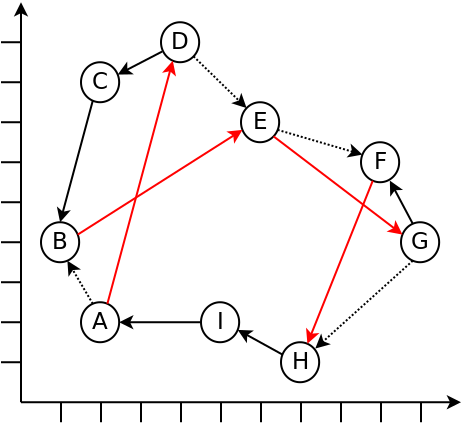
\includegraphics[width=1\linewidth]{figuras/pml/exemplo-rodolfo-2opt-1-3-5-6.png}
        \end{subfigure}
    \end{minipage}
    \begin{minipage}{.475\textwidth}
\begin{Verbatim}[commandchars=\\\{\}]
index:   0  1  2  3  4  5  6  7  8
cidade:  A  \textcolor{green}{D  C  B}  E  \textcolor{blue}{G  F}  H  I
\end{Verbatim}
\begin{gather*}
f(m_2 \circ m_3 \circ s_1): 3734/20487 \ (PCV/PML) \\
f(m_3 \circ m_2 \circ s_1): 3734/20487 \ (PCV/PML) \\
f(m_2 \circ m_3 \circ s_1) = f(m_3 \circ m_2 \circ s_1) \\ \\
\widehat{m_2}(s_1)+\widehat{m_3}(s_1)+f(s_1) = \\
299 + 804 + 2631 = 3734 \ (PCV) \\
1265+6148+13074=20487 \ (PML)
\end{gather*}
    \end{minipage}
    \caption{Solução $m_2 \circ m_3 \circ s_1 = m_3 \circ m_2 \circ s_1$, com $m_2$ sendo 2-opt(5,6) e $m_3$ sendo 2-opt(1,3).}
    \label{fig:figuraExemplo_m2m3s1}
\end{figure}

Note, pela Figura~\ref{fig:figuraExemplo_m2m3s1}, que $m_2 \circ m_3$ opera como um movimento 4-opt (quatro arcos são removidos e inseridos), assim a operação de composição do multi-improvement é capaz de lidar com movimentos de dimensões maiores, em uma única iteração.

\subsubsection{Movimentos conflitantes} \label{subsubsec:movimentosConflitantes}

Há movimentos com conflito de escrita na representação (estrutura de dados) da solução, portanto não é possível aplicá-los simultaneamente. Nesse caso, diz-se que eles são dependentes de ordem (order-dependent moves) ou, simplesmente, conflitantes.

Por exemplo, como $m_1$=2opt(1,7) e $m_3$=2opt(1,3) são conflitantes, $m_1 \circ m_3 \circ s_1$ e $m_3 \circ m_1 \circ s_1$ são soluções estruturalmente distintas, conforme pode ser visto na Figura~\ref{fig:figuraExemplo_m1m3s1}.

\begin{figure}[ht]
    \begin{minipage}{.475\textwidth}
        \begin{subfigure}[t]{1\textwidth} %
            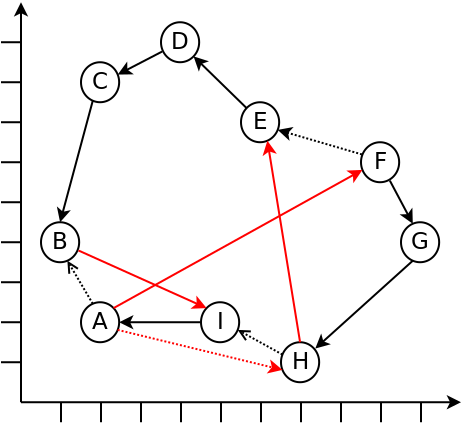
\includegraphics[width=1\linewidth]{figuras/pml/exemplo-rodolfo-2opt-1-7-1-3.png}
        \end{subfigure}
    \end{minipage}
    \begin{minipage}{.475\textwidth}
\begin{Verbatim}[commandchars=\\\{\}]
index:   0  1  2  3  4  5  6  7  8
cidade:  A  \textcolor{red}{H  G  F  E  \textcolor{green}{B  C  D}}  I
\end{Verbatim}
\begin{gather*}
f(m_1 \circ m_3 \circ s_1) : 3700/18395 \ (PCV/PML)\\
\widehat{m_1}(m_3 \circ s_1) + \widehat{m_3}(s_1) + f(s_1) =\\
265+804+2631=3700 \ (PCV) \\
827+6148+13074=18395 \ (PML)
\end{gather*}
    \end{minipage}
    \caption{Solução $m_1 \circ m_3 \circ s_1$, com $m_1$ sendo 2-opt(1,7) e $m_3$ sendo 2-opt(1,3).}
    \label{fig:figuraExemplo_m1m3s1}
\end{figure}

\begin{figure}[ht]
    \begin{minipage}{.475\textwidth}
        \begin{subfigure}[t]{1\textwidth} %
            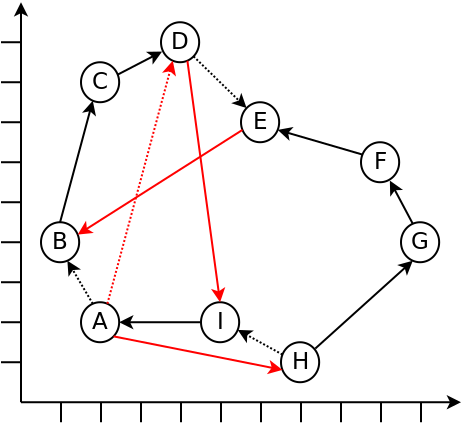
\includegraphics[width=1\linewidth]{figuras/pml/exemplo-rodolfo-2opt-1-3-1-7.png}
        \end{subfigure}
    \end{minipage}
    \begin{minipage}{.475\textwidth}
\begin{Verbatim}[commandchars=\\\{\}]
index:   0  1  2  3  4  5  6  7  8
cidade:  A  \textcolor{green}{F  G  H}  \textcolor{red}{E  D  C  B}  I
\end{Verbatim}
\begin{gather*}
f(m_3 \circ m_1 \circ s_1) = 3728/20403 \ (PCV/PML) \\
\widehat{m_3}(m_1 \circ s_1)+\widehat{m_1}(s_1)+f(s_1) = \\
588+509+2631=3728 \ (PCV) \\
4216+3113+13074=20403 \ (PML)
\end{gather*}
    \end{minipage}
    \caption{Solução $m_3 \circ m_1 \circ s_1$, com $m_3$ sendo 2-opt(1,3) e $m_1$ sendo 2-opt(1,7).}
    \label{fig:figuraExemplo_m3m1s1}
\end{figure}

Naturalmente, como $m_1$ e $m_3$ são conflitantes (vide Figura~\ref{fig:figuraExemplo_m3m1s1}), $\widehat{m_3}(m_1 \circ s_1) \neq \widehat{m_3}(s_1)$ e $\widehat{m_1}(m_3 \circ s_1) \neq \widehat{m_1}(s_1)$.
Também é interessante de notar que a composição executa um movimento 3-opt, então mesmo que não seja permitido na composição do 2-opt pode ser alcançado ao utilizar alguma outra vizinhança num processo simultâneo (generalized multi-improvement).

% Estou achadno a prova do teorema muito fraca
% % Igor coloquei isso aqui como um Teorema, não sei se é muito ambicioso da minha parte
% 
\begin{theorem}[Teorema da independência de movimentos]\label{teo:independenciaMovimentos}
Seja um conjunto $M'$ com movimentos livres de contexto em que todos os movimentos são independentes entre si dois a dois, ou seja $m_i \parallel m_j \mid \forall m_i, m_j \in M'$, com $m_i \ne m_j$.
E seja $s'$ a solução dada pela aplicação de todos os movimentos à solução inicial $s$, logo o valor da solução resultante $s'$ será dado pelo somatório do valor de cada movimento. Assim, pode-se escrever:

% \begin{align*} \label{eq:teo:independenciaMovimentos}
% m_1 \parallel m_2 \implies& s' = m_1 \circ m_2 \circ s \\
% m_1 \parallel m_2 \implies& f(s') = \widehat{m_1}(s) + \widehat{m_2}(s) + f(s) \\
% \end{align*}

% \begin{align*}
\begin{equation}
    \label{eq:teo:independenciaMovimentos}
    \begin{split}
        m_i \parallel m_j, \forall m_i, m_j \in M' \implies& s' = m_1 \circ m_2 \circ \dots \circ m_n \circ s \\
        m_i \parallel m_j, \forall m_i, m_j \in M' \implies& f(s') = f(s) + \widehat{m_1}(s) + \widehat{m_2}(s)+ \widehat{m_3}(s) + \dots + \widehat{m_n}(s) \\
        m_i \parallel m_j, \forall m_i, m_j \in M' \implies& f(s') = f(s) + \sum_i^n{\widehat{m_i}(s)}
    \end{split}
\end{equation}
% \end{align*}
\end{theorem}

\begin{proof}\label{proof:independenciaMovimentos}
% ---
% Prova por contradição
% ---
Suponhamos um conjunto $M = \{ m_1, m_2, \dots, m_n \}$ com $n$ movimentos independentes dois a dois mas $f(m_1 \circ m_2 \circ \dots \circ m_n \circ s) \neq f(s) + \widehat{m_1}(s) + \widehat{m_2}(s)+ \widehat{m_3}(s) + \dots + \widehat{m_n}(s)$.

\begin{align*}
    f(m_1 \circ m_2 \circ \dots \circ m_n \circ s) \neq f(s) + \widehat{m_1}(s) + \widehat{m_2}(s) + \dots + \widehat{m_n}(s) & \\
    \widehat{m_1}(m_2 \circ \dots \circ m_n \circ s) + f(m_2 \circ \dots \circ m_n \circ s) \neq f(s) + \widehat{m_1}(s) + \widehat{m_2}(s) + \dots + \widehat{m_n}(s) & \ [1] \\
    \widehat{m_1}(s) + f(m_2 \circ \dots \circ m_n \circ s) \neq f(s) + \widehat{m_1}(s) + \widehat{m_2}(s) + \dots + \widehat{m_n}(s) & \\
    \widehat{m_1}(s) + \widehat{m_2}(m_3 \circ \dots \circ m_n \circ s) + f(m_3 \circ \dots \circ m_n \circ s) \neq f(s) + \widehat{m_1}(s) + \widehat{m_2}(s) + \dots + \widehat{m_n}(s) & \ [2] \\
    \widehat{m_1}(s) + \widehat{m_2}(s) + f(m_3 \circ \dots \circ m_n \circ s) \neq f(s) + \widehat{m_1}(s) + \widehat{m_2}(s) + \dots + \widehat{m_n}(s) & \\
    \vdots & \\
    \widehat{m_1}(s) + \widehat{m_2}(s) + \dots + \widehat{m_n}(s) + f(s) \neq f(s) + \widehat{m_1}(s) + \widehat{m_2}(s) + \dots + \widehat{m_n}(s) & \ [3] \\
\end{align*}

Os passos acima se dão conforme:
\begin{align*}
[1] \ & m_1 \parallel m_i \mid \forall m_i \in M \\
[2] \ & m_2 \parallel m_i \mid \forall m_i \in M \\
[3] \ & \textrm{Logo temos uma contradição} \bot
\end{align*}

Desta forma, por \textit{reductio ad absurdum} demonstramos que se os movimentos são independentes então o valor da solução resultante se dará pelo somatório da solução anterior com o valor dos movimentos.

% ---
% Indução
% ---
% Pela Equação~\ref{eq:movimentoCustoSomaDois} temos que $f(m_1 \circ m_2 \circ s) = \widehat{m_1}(s) + \widehat{m_2}(s) + f(s)$, supondo por hipótese de indução que $f(m_1 \circ m_2 \circ \dots \circ m_n \circ s) = f(s) + \widehat{m_1}(s) + \widehat{m_2}(s) + \dots + \widehat{m_n}(s)$

% \begin{align*}
%     f(m_1 \circ m_2 \circ \dots \circ m_n \circ m_{n+1} \circ s) = & f(m_{n+1} \circ m_1 \circ m_2 \circ \dots \circ m_n \circ s) \\
%     f(m_1 \circ m_2 \circ \dots \circ m_n \circ m_{n+1} \circ s) = & \widehat{m_{n+1}}(m_1 \circ m_2 \circ \dots \circ m_n \circ s) + f(m_1 \circ m_2 \circ \dots \circ m_n \circ s) \\
% \end{align*}

% % \widehat{m_1}(s) + \widehat{m_2}(s) + \dots + \widehat{m_n}(s) + f(s)
% Fazendo $s_2 = m_2 \circ \dots \circ m_n \circ s$.
% \begin{align*}
%     f(m_1 \circ m_2 \circ \dots \circ m_n \circ m_{n+1} \circ s) = & \widehat{m_{n+1}}(m_1 s_2) + f(m_1 \circ m_2 \circ \dots \circ m_n \circ s) \\
%     f(m_1 \circ m_2 \circ \dots \circ m_n \circ m_{n+1} \circ s) = & \widehat{m_{n+1}}(s_2) + f(m_1 \circ m_2 \circ \dots \circ m_n \circ s)
% \end{align*}

% Pois $m_{n+1} \parallel m_1$, fazendo agora $s_3 = m_3 \circ \dots \circ m_n \circ s$.
% \begin{align*}
%     f(m_1 \circ m_2 \circ \dots \circ m_n \circ m_{n+1} \circ s) = & \widehat{m_{n+1}}(m_2 \circ \dots \circ m_n \circ s) + f(m_1 \circ m_2 \circ \dots \circ m_n \circ s)\\
%     f(m_1 \circ m_2 \circ \dots \circ m_n \circ m_{n+1} \circ s) = & \widehat{m_{n+1}}(m_2 \circ s_3) + f(m_1 \circ m_2 \circ \dots \circ m_n \circ s)\\
%     f(m_1 \circ m_2 \circ \dots \circ m_n \circ m_{n+1} \circ s) = & \widehat{m_{n+1}}(s_3) + f(m_1 \circ m_2 \circ \dots \circ m_n \circ s)\\
%     \vdots \\
%     f(m_1 \circ m_2 \circ \dots \circ m_n \circ m_{n+1} \circ s) = & \widehat{m_{n+1}}(s) + f(m_1 \circ m_2 \circ \dots \circ m_n \circ s)\\
%     f(m_1 \circ m_2 \circ \dots \circ m_n \circ m_{n+1} \circ s) = & \widehat{m_{n+1}}(s) + \widehat{m_1}(s) + \widehat{m_2}(s) + \dots + \widehat{m_n}(s) + f(s)
% \end{align*}

% Logo, por indução finita temos que $m_i \parallel m_j, \forall m_i, m_j \in M' \implies f(s') = f(s) + \sum_i^n{\widehat{m_i}(s)}$.

\end{proof}


\subsection{First Improvement vs Best Improvement} \label{subsec:firstBestImprovement}

As estratégias \textit{First Improvement} (Primeira melhora) e \textit{Best Improvement} (Melhor melhora) recebem como parâmetro a solução da iteração corrente para gerar seus vizinhos e escolhem uma solução a ser retornada conforme um critério específico, a saber, a primeira solução a melhorar a atual e a melhor solução encontrada na vizinhança, respectivamente.

\begin{algorithm}[htpb]
\caption{First Improvement para um problema de minimização}
\label{alg:firstImprovement}
\begin{algorithmic}[1]
    \Function{FirstImprovement}{Solução: $s$, Operador de vizinhança: $x$}
        % \For{$s' \in N^x(s)$} \Comment{Para cada solução $s'$ vizinha de $s$}
        %     \If{$f(s') < f(s)$} \Comment{Se a solução for melhor que a atual}
        %         \Return{$s'$}
        %     \EndIf
        % \EndFor
        \For{$m_i \in M$} \Comment{Para cada movimento $m_i \in M$}
            \If{$\widehat{m_i}(s) < 0$} \Comment{Se a solução for melhor que a atual}
                \Return{$m_i \circ s$}
            \EndIf
        \EndFor
        \Return{$s$} \Comment{Caso não consiga melhorar retorna a própria solução}
    \EndFunction
\end{algorithmic}
\end{algorithm}

Podemos ver o pseudocódigo do \textit{First Improvement} no Algoritmo~\ref{alg:firstImprovement} que consiste de enumerar os vizinhos até encontrar o primeiro que seja melhor que a solução atual, este então é retornado como resposta do método.
O método de \textit{Best Improvement} (Algoritmo~\ref{alg:bestImprovement}) consiste em enumerar toda a vizinhança guardando a informação do melhor encontrado até o momento, e então retornar o melhor resultado encontrado.

\begin{algorithm}[htpb]
\caption{Best Improvement para um problema de minimização}
\label{alg:bestImprovement}
\begin{algorithmic}[1]
    \Function{BestImprovement}{Solução: $s$, Operador de vizinhança: $x$}
        % \Let{$s^{best}$}{$s$} \Comment{Melhor solução encontrada}
        % \For{$s' \in N^x(s)$} \Comment{Para cada solução $s'$ vizinha de $s$}
        %     \If{$f(s') < f(s)$} \Comment{Se a solução for melhor que a atual altera a melhor solução encontrada}
        %         \Let{$s^{best}$}{$s'$}
        %     \EndIf
        % \EndFor
        \Let{$s^{best}$}{$s$} \Comment{Melhor solução encontrada}
        \For{$m_i \in M$} \Comment{Para cada movimento $m_i \in M$}
            \If{$\widehat{m_i}(s) < f(s^{best}) - f(s)$} \Comment{Se a solução for melhor que a atual altera a melhor solução encontrada}
                \Let{$s^{best}$}{$m_i \circ s$}
            \EndIf
        \EndFor
        \Return{$s^{best}$} \Comment{Retorna a melhor solução encontrada}
    \EndFunction
\end{algorithmic}
\end{algorithm}

O \textit{First Improvement} pode ser uma opção ao método de \textit{Best Improvement} quando a enumeração de toda a vizinhança é uma atividade muito custosa.
% Posso afirmar isso?
Embora não haja um paralelo para a definição matemática formal da solução $s'$ retornada pelo \textit{First Improvement} esta pode ser definida para o \textit{Best Improvement} de maneira simples por $s' \in N^x(s) \mid f(s') < f(s), \forall s \in N^x(s)$, o que, como veremos a seguir na seção~\ref{sec:otimoLocalGlobal}, corresponde ao ótimo local para a solução $s$ segundo a vizinhança $x$.
Em termos de movimento temos $s' = m' \circ$ com $\widehat{m'}(s) < \widehat{m_i}(s) \mid \forall m_i \in M$.

\subsection{Random Selection}

Nesta estratégia \textit{Random Selection} (Escolha Aleatória) é selecionada uma solução aleatoriamente entre aquelas que melhoram a solução atual.

\begin{algorithm}[htpb]
\caption{Random Selection para um problema de minimização}
\label{alg:randomSelection}
\begin{algorithmic}[1]
    \Function{RandomSelection}{Solução: $s$, Operador de vizinhança: $x$}
        \Let{$S_{imp}$}{$\emptyset$} \Comment{Conjunto com soluções de melhora}
        \For{$m_i \in M$} \Comment{Para cada movimento $m_i \in M$}
            \If{$\widehat{m_i}(s) < 0$} \Comment{Se a solução for melhor que a atual}
                \Let{$S_{imp}$}{$S_{imp} \cup \{ m_i \circ s\}$} \label{alg:randomSelection:salvaMelhora} \Comment{Adiciona ao conjunto de soluções de melhora}
            \EndIf
        \EndFor
        \Return{$Any(S_{imp})$} \Comment{Retorna uma das soluções de melhora}
    \EndFunction
\end{algorithmic}
\end{algorithm}

A estratégia \textit{Random Selection} (mostrada no Algoritmo~\ref{alg:randomSelection}) navega pelas soluções e na mantém as melhores soluções que melhoram a solução atual, conforme linha~\ref{alg:randomSelection:salvaMelhora}, para ao final retornam uma deste grupo.

\subsection{Multi Improvement}

Uma alternativa ao \emph{Best Improvement}, \emph{First Improvement} e ao \emph{Random Selection} é o \emph{Multi Improvement}~\cite{rios2015}.
A ideia é combinar um conjunto de movimentos independentes e executá-los simultaneamente sobre a solução de entrada.
Note que, embora consista na aplicação de diversos movimentos, somente uma única solução vizinha é gerada.
O \emph{Multi Improvement} pode ser utilizado em qualquer contexto que o \emph{Best Improvement} ou \emph{First Improvement} se encaixe (etapa de Exploração de Vizinhança ou {\it Neighborhood Exploration}), porém caso só exista um único movimento independente na vizinhança, ele terá comportamento equivalente ao Best Improvement.
Assim a solução $s'$ retornada por uma iteração do \emph{Multi Improvement} após ser aplicado a uma solução $s$ é dada por $s' = m_1 \circ m_2 \circ \dots m_k \circ s$ com os movimentos independentes $\{ m_1, m_2, \dots, m_k \} \subset M$.

O \emph{Multi Improvement} se encaixa particularmente bem com o conceito de \emph{SIMD} (\emph{Single Instruction Multiple Data}), presente nas GPUs, sendo sua complexidade similar ao \emph{Best Improvement} (todos movimentos da vizinhança são enumerados), seguido de uma etapa de junção (ou {\it merge}) dos movimentos independentes.
Podem existir cenários em que o \emph{Best Improvement} seja mais eficiente (com poucos movimentos independentes), embora já tenha sido demonstrado na literatura que mesmo casos com apenas dois movimentos independentes acabam mais promissores no \emph{Multi Improvement} do que no \emph{Best Improvement}. % Não seria importante colocar a referência disso?

\subsection{Passo iterativo} \label{subsec:passoIterativo}
% Posso fazer essa definição que estou fazendo aqui?
% Pensei em fazer isso para facilitar explicar algumas coisas mais pra frente

Em geral, um algoritmo de busca local é um processo iterativo pesado que tem como objetivo encontrar uma solução melhor que a atual dentro de um espaço de busca.
A solução recebida como entrada pode ser aleatória ou advinda de alguma heurística construtiva, a intenção do processo é aprimorar o resultado encontrado.

Cada iteração da busca local tenta encontrar a melhor solução mediante alguma alteração na solução atual, então o processo se repete na solução gerada até que nenhuma melhora seja possível.

\begin{algorithm}[htpb]
\caption{Busca local definida de forma genérica}
\label{alg:localSearch}
\begin{algorithmic}[1]
    \Function{LocalSearch}{Solução: $s$}
        \While{$f(Alterar(s)) < f(s)$} \Comment{Cada iteração corresponde a um passo iterativo da busca local}
            \Let{s}{$Alterar(s)$}
        \EndWhile
        \Return{$s$} \Comment{Retorna a melhor solução encontrada}
    \EndFunction
\end{algorithmic}
\end{algorithm}

Supondo que $Alterar(s)$ (apresentado do Algoritmo~\ref{alg:localSearch}) retorna uma solução melhor que a atual segundo alguma alteração, convencionemos então chamar de \textbf{passo iterativo} cada iteração da busca local em que o processo obtém uma solução melhor que a atual e salva o melhor resultado encontrado até o momento.
Assim para uma solução $s$ o passo iterativo é dado pela Equação~\ref{eq:passoIterativo}.

\begin{equation} \label{eq:passoIterativo}
\rho(s) = min(s, Alterar(s)) \implies f(\rho(s)) \le f(s)
\end{equation}

\section{Ótimo global vs Ótimo local} \label{sec:otimoLocalGlobal}

O ótimo global e ótimo local são exemplificados na Figura~\ref{fig:espacoDeBusca}.
Uma solução $s^* \in S$ é dita \textbf{ótimo global} para um problema $\Pi$ quando não existe outra solução viável $s'$ com melhor valor de função objetivo, formalmente temos que $s^*$ é ótimo global quando:
\begin{itemize}
    \item $\forall s' \in S \mid f(s') \le f(s^*), s' \neq s^* $ para um problema de maximização;
    \item $\forall s' \in S \mid f(s') \ge f(s^*), s' \neq s^* $ para um problema de minimização.
\end{itemize}

Considere uma busca local de \textit{Best Improvement} $H$ para o problema $\Pi$ sobre a estrutura de vizinhança $N^x$, após aplicar $H$ a uma solução inicial $s^0 \in S$ é obtido um conjunto de soluções $N^x(s^0)$ vizinhas, assim o \textbf{ótimo local} (\textit{mínimo local}) segundo a vizinhança $N^x$ para a solução $s^0$ é dado por:
\begin{itemize}
    \item $s'' \in N^x(s^0) \mid f(s'') < f(s'), \forall s' \in N^x(s^0), s'' \neq s'$, para um problema de minimização;
    \item $s'' \in N^x(s^0) \mid f(s'') > f(s'), \forall s' \in N^x(s^0), s'' \neq s'$, para um problema de maximização.
\end{itemize}

Em linhas gerais um \textbf{ótimo local} é a solução com melhor valor de função objetivo para um contexto local, seja uma vizinhança ou o conjunto imagem de uma heurística.

\section{Meta-heurísticas} \label{sec:metaHeuristicas}

Uma meta-heurísticas diferencia-se de uma heurística por não ser acoplada a um problema específico ou classe de problemas.
Meta-heurísticas fazem uso de artifícios capazes de encontrar soluções e aprimorar as já encontradas enquanto procuram escapar de mínimos locais.
Na literatura são utilizadas em trabalhos que tratam de problemas da classe NP-Difícil devido a simplicidade de implementação e a intratabilidade da solução exata de tais problemas.
Assim, esses algoritmos são ferramentas robustas para serem aplicadas na resolução prática de problemas de otimização combinatória, sendo uma alternativa quando o respectivo algoritmo exato não é conhecido ou exige um alto tempo de execução \cite{glover2006handbook}.

As meta-heurísticas evoluem iterativamente conforme a parametrização fornecida até atingir um \textbf{Critério de Parada}, que pode também estar sujeito aos parâmetros do método.
O critério de parada, em geral, está associado ao número de iterações, tempo de execução, um parâmetro de qualidade ou número de iterações sem melhora.

\section{Dataflow} \label{sec:conceitosDataflow}
% Essa parte tá bem próxima da tese do Marzulo

Atualmente os processadores no mercado de computadores seguem, em geral, o modelo de \textit{Von Neumann}.
No referido modelo, a execução das instruções é guiada por um fluxo de controle, ou seja, segundo a ordem que aparecem no programa, desta forma se faz necessário um \textit{Program Counter} (Contador de Programa) para indicar qual a próxima instrução a ser executada.
O contador também pode ser alterado por instruções de desvio, e laços de repetição ou qualquer tipo de comando de execução condicional.

Note que este modelo é intrinsecamente sequencial. No entanto, tenta-se resgatar paralelismo em nível de instruções com técnicas como pipelining~\cite{patterson2003computerOrganization}, predição de desvio~\cite{patterson2003computerOrganization} e renomeamento de registradores~\cite{patterson2012}.

O modelo dataflow~\cite{2468, Swanson2003, 642111, Davis:1978:ASM:800094.803050, 714523, Shimada:1986:EPD:17356.17383, Kishi:1983:DDD:1067651.801661, Grafe:1989:EDP:74925.74930, 134511, Swanson:2007:WA:1233307.1233308} expõe paralelismo de forma natural.
Neste modelo, as instruções são executadas de acordo com o fluxo de dados, ou seja, assim que todos os seus operandos de entrada estiverem disponíveis.

No modelo dataflow os programas são escritos como um grafo de fluxo de dados onde os nós representam as instruções e as arestas direcionadas indicam as dependências de dados.
Assim $A \rightarrow B$ indica que $A$ produz um dado que é enviado como entrada para $B$ após ter sido processado.
Cabe lembrar que este modelo é adotado nas máquinas de Von Neumann para extrair paralelismo ao implementar o mecanismo de execução fora-de-ordem com escalonamento dinâmico baseado em fluxo de dados~\cite{tomasulo}, contudo limitado o paralelismo pela emissão das instruções que permanece seguindo o fluxo de controle.
Numa arquitetura que segue totalmente o fluxo de dados as instruções não são emitidas segundo se apresentam no programa, instruções distintas podem executar concorrentemente.

Na Figura~\ref{fig:dataflowExemploPython} pode ser visto um programa simples, à esquerda é mostrado o código e à direita sua tradução no grafo de fluxo de dados associado, note que as instruções de soma e multiplicação podem ser executadas em paralelo ou qualquer ordem sem alterar o resultado final.

\begin{figure}
    \centering
    \begin{minipage}{.3\textwidth}
        \centering
\begin{minted}{python}
a = 10
b = 9
c = 3
d = 8
e = a * b
f = c + d
if e > f:
  g = (a - b) * a
else:
  g = (c - d) * d
\end{minted}
    \end{minipage}
    \begin{minipage}{.675\textwidth}
        \centering %width=.655\linewidth
        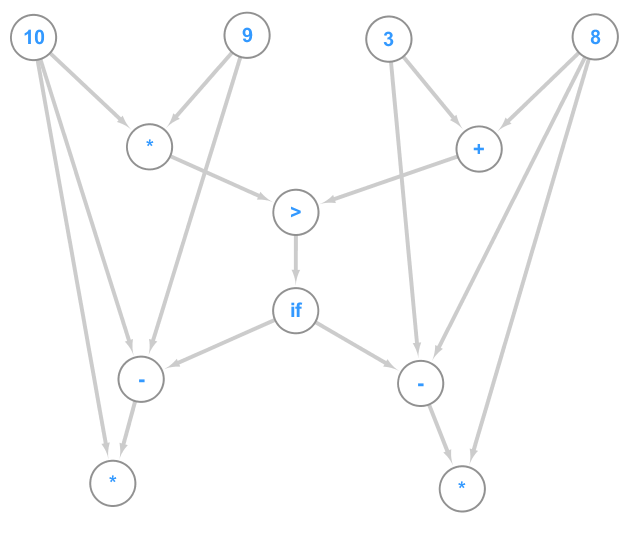
\includegraphics[scale=.7]{figuras/dataflow/pythonCodeDf.png}
    \end{minipage}
    \caption{Exemplo de conversão código para grafo de dependências.
    À esquerda pode ser visto um trecho de código em \emph{python} ao passo que à direita é exibido o grafo dataflow associado.}
    \label{fig:dataflowExemploPython}
\end{figure}

\subsection{Sucuri} \label{sect:sucuri}

Sucuri~\cite{sucuri-original} é uma biblioteca minimalística Dataflow para a linguagem Python que permite aos programadores explorarem o paralelismo mais naturalmente pela execução dataflow em máquinas que seguem a arquitetura Von Neumann.
Sucuri permite uma execução transparente em um \emph{cluster} de máquinas ao fazer uso do mecanismo de serialização de objetos em Python (\emph{Pickle}).

Conceitualmente, um grafo dataflow é composto de nós que representa tarefas, que podem ser de grão fino (como instruções) ou grão grosso (como funções ou procedimentos).
As arestas que conectam os nós representam dependências de dados, significando que um nó de origem irá produzir um resultado que será utilizado por um nó de destino.
Quando um certo nó recebe todas as entradas necessárias (são satisfeitas todas as suas dependências) este pode ser enfileirado para executar o seu processamento.

A Figura~\ref{fig:arch} mostra a estrutura do Sucuri, onde é possível observar três componentes principais:
\texttt{Graph} (Grafo), \texttt{Scheduler} (Escalonador) e o \texttt{Worker} (Operário).

O \texttt{Graph} é apenas o grafo de dependências da aplicação dataflow, podendo ser visto como um contêiner de nós, onde cada um contêm:
\begin{itemize}
    \item{A lista de entradas de dados até o momento.
    Quando todos os operandos são recebidos ocorre um \emph{matching} e a execução do nó será disparada;}
    \item{A função (computação) que deve ser executada quando for o momento para este nó;}
    \item{Uma lista de nós de destino que devem receber o resultado produzido na sua computação;}
    \item{Atributos específicos, como um identificador único que pode ser usado para atribuição de trabalho para um conjunto específico de nós (como numa abordagem \emph{fork-join}).}
\end{itemize}

Quando é usado em um \emph{cluster} de computadores, cada componente supracitado é replicado em cada máquina do \emph{cluster}, com exceção do \texttt{Scheduler}, o que implica que a Sucuri adota um \emph{pool} de tarefas centralizado.
Em~\cite{sucuri-distribuida} os autores da Sucuri implementaram e avaliaram uma versão da biblioteca utilizando um escalonador distribuído, contudo esta versão ainda não foi utilizada nesse trabalho.

\begin{figure}[htbp]
    \centering
    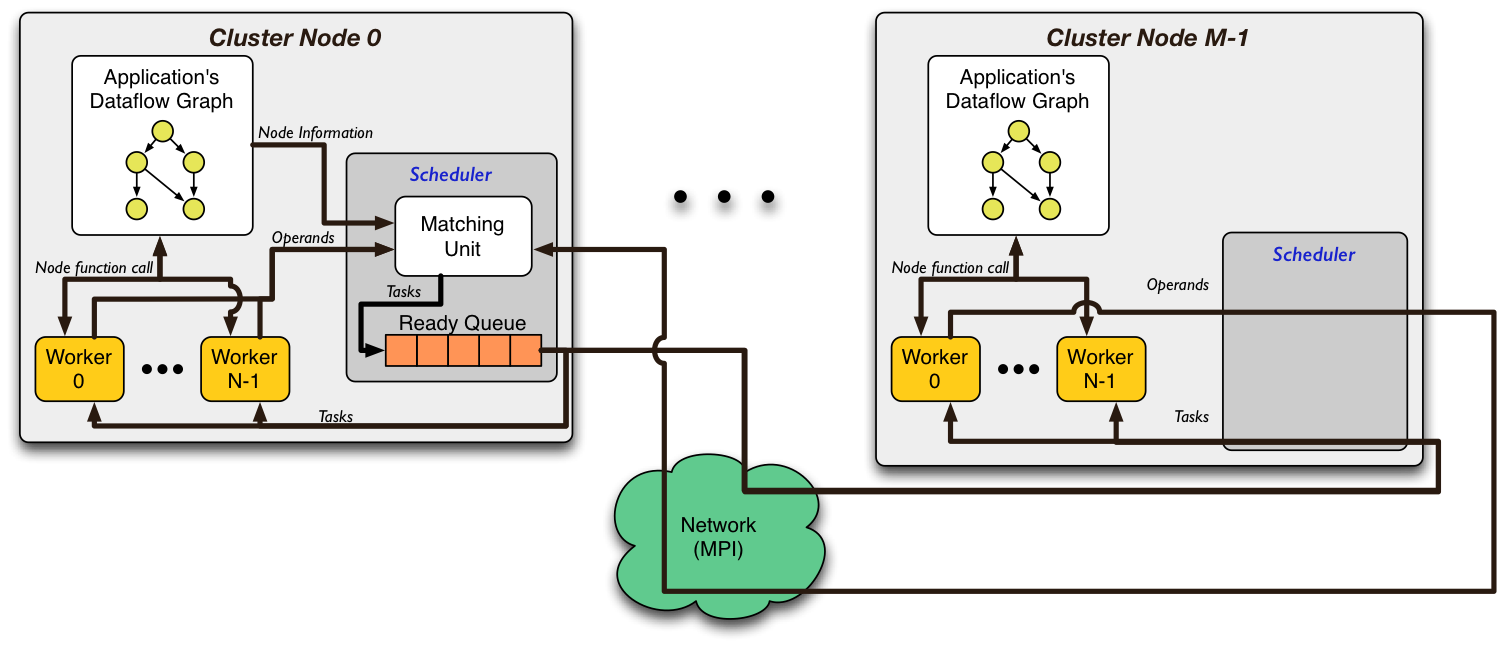
\includegraphics[scale=0.65]{figuras/dataflow/SucuriArchitectureHorizonal.png}
    \caption{A Arquitetura da Sucuri (de~\cite{sucuri-original}).
    A mesma estrutura é replicada em cada nó, entretanto apenas no \texttt{Scheduler} do nó 0 do cluster contem o \texttt{Matching Unit} e o \texttt{Ready Queue}.
    Este é responsável por receber operandos dos \texttt{workers} locais e de outros \texttt{Schedulers}, além disso este gera as tarefas para serem enfileiradas no \texttt{Ready Queue}.}
    \label{fig:arch}
\end{figure}

O \texttt{Scheduler} (escalonador) principal, situado no nó 0 do \emph{cluster}, é composto por uma \texttt{Matching Unit}, uma \texttt{Ready Queue} (fila de prontos) e uma \texttt{Waiting Queue} (fila de espera).
Este é responsável por entregar todos os operandos aos seus respectivos nós de destino no grafo.
Se ocorre um \emph{match}, isto é, todas as dependências de dados são satisfeitas para um nó, então uma tarefa é criada e inserida na \texttt{Ready Queue}.
Quando os \texttt{workers} estiverem ociosos estes vão requisitar uma tarefa para o \texttt{Scheduler} que será buscada da \texttt{Ready Queue}.
O \texttt{Scheduler} situado em outros nós do cluster são mais simples e apenas encaminham tarefas do \texttt{Scheduler} principal para seus \texttt{workers} locais e operandos de seus \texttt{workers} para o \texttt{Scheduler} principal.
O grafo é replicado em todos os nós do \emph{cluster} mas apenas o grafo do nó 0 pode receber operandos do \texttt{Scheduler} principal.

Toda a comunicação intra-nó entre os componentes principais citados acima é realizada via memória compartilhada e entre \texttt{Schedulers} de nós diferentes é feita via interface.

Cada nó do grafo da Sucuri é associado a uma função que pode ser implementada pelos programadores e passada para estes no momento da criação do grafo dataflow.
Após instanciar os nós, o programador pode criar as ligações entre estes usando o método \texttt{add\_edge()} do nó que cria uma dependência no grafo dataflow.
Quando o escalonador dispara a execução de uma tarefa num certo worker, este vai chamar a execução do método \texttt{run()} do respectivo nó para aquela tarefa.
Na maioria dos casos, este método \texttt{run()} vai atuar como um invólucro que chama a execução da função associada ao nó no momento da construção do grafo, passando os operandos como parâmetro e ao final irá enviar os valores retornados pela função para o escalonador.

De mais a mais Sucuri também provê um conjunto especial de nós que podem auxiliar o programador a elaborar aplicações que sigam alguns padrões de paralelismo.
Por exemplo, uma aplicação que envolva \emph{pipeline} para Sucuri é apresentada na Figura~\ref{fig:pipeline}.
O painel $A$ mostra o grafo representando este padrão e o painel $B$ o código Sucuri para essa operação.
Note como novos nós são criados (linhas 11-13), adicionados ao grafo (linhas 17-19) e como as arestas conectando os nós são definidas (linhas 21 e 22).
Perceba também a instanciação no escalonador (linha 6) e como este é inicializado após o grafo dataflow ter sido definido (linha 23).

A Figura~\ref{fig:pipeline} também aponta como o nó especial \texttt{Source} recebe um objeto \emph{iterador} Python (por exemplo uma lista ou um descritor de arquivo) na sua instanciação.
Durante a execução do programa, o método \texttt{run()} do nó \emph{Source} será disparado apenas uma vez visto que este é a raiz, i.e., não possui operandos de entrada no grafo e é usado para iniciar a computação.
Todavia, a execução deste método vai durar até que todo o conteúdo do objeto iterador tenha sido consumido.
Por padrão o nó \texttt{Source} vai executar um laço sobre o objeto iterador e produzirá múltiplas saídas (mensagens) que irão disparar a execução do pipeline múltiplas vezes.

Veja também que o último nó do pipeline é o nó especial \texttt{Serializer}, que é responsável por escrever os dados no arquivo.
É possível que os dados produzidos pelo nó \texttt{Source} sejam processados fora de ordem pelo segundo nó uma vez que múltiplas tarefas podem ser escalonadas em workers diferentes.
Por conseguinte, é necessário reordenar os dados antes de os escrever no arquivo, no nó \texttt{Serializer}.
Para tanto, os dados produzidos pelo nó \texttt{Source} precisam estar encapsulados num objeto \texttt{TaggedValue} que contem uma atributo \texttt{tag}, indicando sua posição na ordem do conjunto de dados.
O nó no intermédio também vai enviar os dados filtrados dentro do objeto \texttt{TaggedValue}, com a mesma tag do pedaço de dados que recebeu.
O nó \texttt{Serializer} então ao receber os dados do nó de filtro, vai armazená-los num \emph{buffer} ordenando de acordo com a tag.
Se a tag do último fragmento de dados recebido corresponde ao próximo a ser escrito no arquivo então o nó \texttt{Serializer} obtém os dados do \emph{buffer} ordenando e escreve no arquivo até que haja uma lacuna na ordenação, i.e. a porção de dados que é a próxima a ser escrita ainda não chegou ao \emph{buffer}.
Se os dados recebidos pelo \texttt{Serializer} estão fora de ordem, o nó apenas os armazena no \emph{buffer} ordenado e aguarda por mais dados.
O método \texttt{pin\(\)} é usado para fixar um nó a um determinado worker, o que fará com que este seja executado apenas por este worker específico.
No caso do exemplo, foram fixados os nós que fazem operações de E\/S no disco aos workers que tem acesso direto ao disco.

\begin{figure}[htbp]
    \centering
    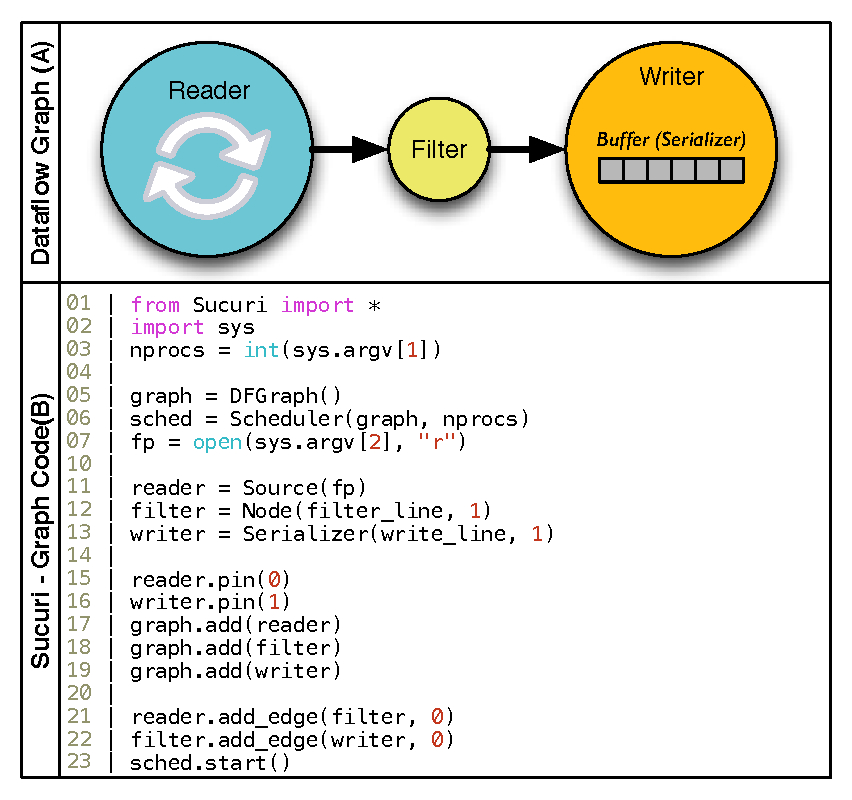
\includegraphics[scale=0.75]{figuras/dataflow/pipeline.eps} 
    \caption{\emph{Pipelining} com Sucuri. 
    %The data is read from the disk by \texttt{Reader} node encapsulated in a \texttt{TaggedValue} object while a filter is applied by \texttt{Filer} node in a data read previously. As the \texttt{Filter} finish, the \texttt{Writer} node receives and store them in buffer sorted according to the tag. If the tag of the last piece of data received corresponds to the next data to be written to the file, the \texttt{Writer} node proceeds to pop data from the sorted buffer and write to the file.
    Painel $A$ mostra um grafo de uma aplicação dataflow, o painel $B$ descreve o grafo usando a Sucuri.}
    \label{fig:pipeline}
\end{figure}

Um recurso de modelagem interessante que foi usado nesse trabalho consiste em explorar a programação em grão grosso usando a Sucuri junto com a computação em grão fino em GPU, resultando assim numa computação heterogênea Dataflow/Von Neumann, com nós dataflow executando operações de alta performance em GPU.
Esta estratégia permite uma grande flexibilidade para o design de insólitos algoritmos, com maior simplicidade do que adotando um único paradigma de computação (dataflow ou Von Neumann).

\section{RVND} \label{sec:rvndClassico}

O método RVND clássico~\cite{souza2010} é apresentado no Algoritmo~\ref{alg:rvnd}, como um procedimento sequencial, este depende do passo anterior para continuar o seu processamento, de acordo com o resultado anterior o método pode decidir se move para a próxima vizinhança ou volta para a primeira.
Podemos ver no condicional da linha \ref{alg:rvndTeste} que após obter a melhor solução para a vizinhança atual, o RVND verifica se esta é melhor que a solução atual, caso seja então o método volta pra a primeira vizinhança, caso contrário segue para a seguinte.

\begin{algorithm}[htpb]
\caption{RVND clássico}
\label{alg:rvnd}
\begin{algorithmic}[1]
    \Function{RVND}{Solução: $s$}
        \Let{$N$}{$\{N^1,\dots,N^{kmax}\}$} \Comment{Vizinhanças em ordem aleatória}
        \For{$k \leftarrow 1$ to $kmax$}
            \Let{$s'$}{ $s''$ com $f(s'') \le f(s''') \mid \forall s''' \in N^k(s)$} \Comment{Melhor solução de $N^k(s)$}
            
            \If{$f(s') < f(s)$} \label{alg:rvndTeste}
                \Let{$s$}{$s'$}
                \Let{$k$}{$1$}
            \Else
                \Let{$k$}{$k + 1$}
            \EndIf
        \EndFor
        \Return{s'}
    \EndFunction
\end{algorithmic}
\end{algorithm}

A cada iteração o RVND retorna uma solução $s' = m_y^x$ com $\widehat{m_y^x}(s) < \widehat{m_i^x}(s) \mid \forall m_i^x \in M^x$, que corresponde à melhor solução para a vizinhança atual.

% \mathscr{M}
Considerando $ \mathcal{M} = M^{RVND} = M^1 \cup M^2 \cup \dots \cup M^k $ o conjunto com os movimentos de todas as vizinhanças usadas pelo RVND, então em termos de movimento temos que a solução $s''$ retornada ao final do RVND pode ser escrita como $s'' = m_z \circ s$ com $m_z \in \mathcal{M}$ e $\widehat{m_z}(s) < \widehat{m_i}(s) \mid \forall m_i \in \mathcal{M}$.

\section{DVND} \label{sec:dvndClassico}

O \textit{Distributed Variable Neighborhood Descent} DVND concebido por~\cite{RIOS201839} utiliza múltiplas vizinhanças conforme o faz o VND (\textit{Variable Neighborhood Descent} proposto por \cite{mladenovic1997}) contudo propõe o processamento das vizinhanças de forma distribuída.
Este processamento distribuído se dá pelo escalonamento das tarefas de enumeração das vizinhanças o que naturalmente proporciona a aleatoriedade proposta no RVND.

A implementação em dataflow não pode alcançar uma grande melhoria do RVND em termos de tempo ou qualidade da solução pois o grafo se assemelha a uma cascata (veja a Figura~\ref{fig:rvndGraph}) o que não permite alcançar paralelismo, então se torna natural o uso do método DVND conforme o Algoritmo~\ref{alg:dvnd}. 
A ideia do DVND é que quando uma solução atinge um ótimo local para uma estrutura de vizinhança ainda pode existir um vizinho com melhor valor de função objetivo em uma estrutura de vizinhança diferente, destarte não necessariamente sendo um ótimo local para todas as vizinhanças
Se uma melhoria é encontrada o processo de busca é reiniciado para todas as estratégias de vizinhança.

\begin{algorithm}[htpb]
\caption{DVND clássico}\label{alg:dvnd}
\begin{algorithmic}[1]
    \Function{DVND}{Solução: $s$, Vizinhanças: $N$}
        \Let{$W$}{$\emptyset$}
        \Let{$H$}{$\emptyset$}
        \ForAll{$N_k \in N$}
            \Let{$s_k$}{$s$} \Comment{Solução atual para vizinhança $k$}
            \Let{$H_{k,s}$}{$true$} \Comment{Solução já foi enumerada pela vizinhança}
            \Let{$W_k$}{$false$} \Comment{Vizinhança aguardando solução}
            \State Chame de forma assíncrona $N^k(s_k)$
        \EndFor
        
        \While{$\exists w \in W \mid w = false$}
            \Let{$k$}{join $N^k(s_k)$} \Comment{Aguarda a resposta da vizinhança $N^k$}
            \Let{$s_k$}{Melhor solução de $N^k(s_k)$}
            \If{$f(s_k) < f(s)$}
                \Let{$s$}{$s_k$}
            \EndIf
            
            \Let{$W_k$}{$true$}
            \ForAll{$N_k \in N$}
                \If{$W_k \land \neg H_{k,s}$}
                    \Let{$s_k$}{$s$}
                    \Let{$H_{k,s}$}{$true$}
                    \Let{$W_k$}{$false$}
                    
                    \State Chame de forma assíncrona $N^k(s_k)$
                \EndIf
            \EndFor
        \EndWhile
        \Return{$s$}
    \EndFunction
\end{algorithmic}
\end{algorithm}

Considerando $ \mathcal{M} = M^{DVND} = M^1 \cup M^2 \cup \dots \cup M^k $ o conjunto com os movimentos de todas as vizinhanças usadas pelo DVND, então em termos de movimento temos que a solução $s''$ retornada a cada iteração do DVND pode ser escrita como $s'' = m_z \circ s$ com $m_z \in \mathcal{M}$ e $\widehat{m_z}(s) < \widehat{m_i}(s) \mid \forall m_i \in \mathcal{M}$.
Vale ressaltar que $\mathcal{M} = M^{DVND} = M^{RVND}$, a diferença dos métodos é que a cada iteração o RVND move para a melhor solução da vizinhança atual e no caso do DVND este move para a melhor solução entre todas as vizinhanças.

% Igor, o que acha dessa afirmação?
Numa análise em mais alto nível do RVND (Algoritmo~\ref{alg:rvnd}) e DVND (Algoritmo~\ref{alg:dvnd}), pensando-se à luz das estratégias de \textit{First improvement} e \textit{Best improvement}, o RVND enumera as soluções vizinhas da solução atual vizinhança por vizinhança até encontrar uma solução que a melhore e então retorna para a primeira vizinhança ao passo que o DVND enumera todas as vizinhanças para então optar pela solução de melhor valor.
Desta forma o RVND é uma estratégia de \textit{first improvement} no contexto de vizinhanças de solução e o DVND uma estratégia de \textit{best improvement}.
